\def\tightlist{}
\documentclass{deltares_report}
\usepackage{booktabs}
\usepackage{tabu}
$if(highlighting-macros)$
$highlighting-macros$
$endif$
$if(csl-refs)$
% Pandoc citation processing
\newlength{\cslhangindent}
\setlength{\cslhangindent}{1.5em}
\newlength{\csllabelwidth}
\setlength{\csllabelwidth}{3em}
\newlength{\cslentryspacingunit} % times entry-spacing
\setlength{\cslentryspacingunit}{\parskip}
% for Pandoc 2.8 to 2.10.1
\newenvironment{cslreferences}%
  {$if(csl-hanging-indent)$\setlength{\parindent}{0pt}%
  \everypar{\setlength{\hangindent}{\cslhangindent}}\ignorespaces$endif$}%
  {\par}
% For Pandoc 2.11+
\newenvironment{CSLReferences}[2] % #1 hanging-ident, #2 entry spacing
 {% don't indent paragraphs
  \setlength{\parindent}{0pt}
  % turn on hanging indent if param 1 is 1
  \ifodd #1
  \let\oldpar\par
  \def\par{\hangindent=\cslhangindent\oldpar}
  \fi
  % set entry spacing
  \setlength{\parskip}{#2\cslentryspacingunit}
 }%
 {}
\usepackage{calc}
\newcommand{\CSLBlock}[1]{#1\hfill\break}
\newcommand{\CSLLeftMargin}[1]{\parbox[t]{\csllabelwidth}{#1}}
\newcommand{\CSLRightInline}[1]{\parbox[t]{\linewidth - \csllabelwidth}{#1}\break}
\newcommand{\CSLIndent}[1]{\hspace{\cslhangindent}#1}
\renewcommand{\FrontCover}{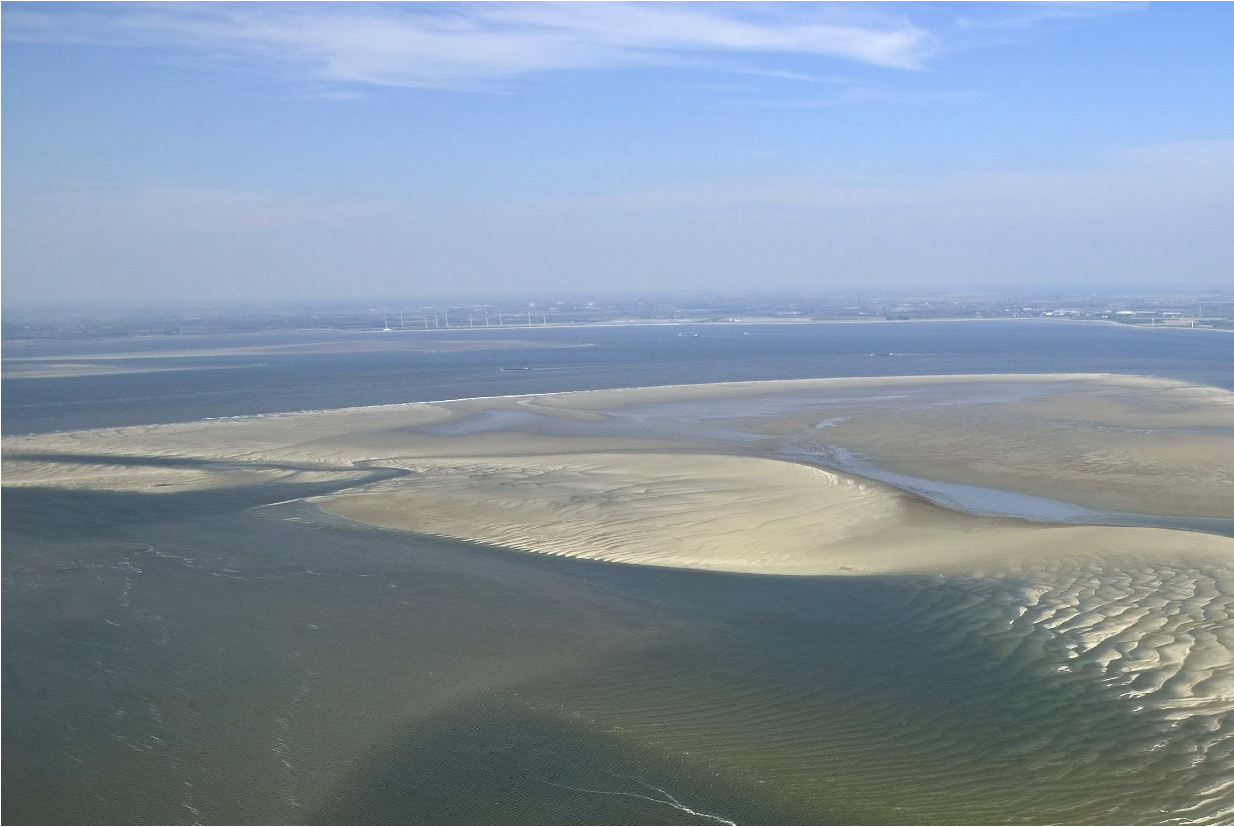
\includegraphics[width=182mm,height=182mm]
{images/cover/getijdenland.pdf}}
\coverPhoto{}
$endif$
\begin{document}
\title{Systeemrapportage Waddenzee abiotiek}
\subtitle{}
\author{Deltares}
\partner{}

\client{Rijkswaterstaat WVL, Rijkswaterstaat Noord-Nederland}
\contact{Martijn Klein Obbink}
\reference{}
\keywords{hydrodynamiek, waterkwaliteit, zwevend stof, sediment, biota, fytoplankton}

\version{2021}
\date{16-08-2022}
\projectnumber{}
\documentid{}
\status{concept}
\disclaimer{}
% \references{}

\authori{Willem Stolte}
\organisationi{Deltares}
\authorii{Jasper Dijkstra}
\organisationii{Deltares}
\authoriii{Julia Vroom}
\organisationiii{Deltares}
\authoriv{Giorgio Santinelli}
\organisationiv{Deltares}
\versioni{0.9}
\revieweri{}
\approvali{Toon Segeren}
\publisheri{Deltares}

\summary{
}
\deltarestitle
%------------------------------------------------------------------------------

% Text body

$body$

%------------------------------------------------------------------------------
\end{document}
